\section{An exact boundary for rates on the old support}
The search over supports below also exposed a small amount of slack in the sufficient mark test itself. Its effect can be isolated without changing a single occupied residue. This comparison matters because an upper theorem for a convenient certificate can appear contradicted by a new witness that uses a slightly better certificate. Here both endpoints can be computed.

For one starting point the source offers on the order of \((h+3)10^{6r+1}\log x\) trials to locate a successful tile. Its dimension exponent on these hosts is \(h=2+8\varepsilon\). A tile containing \(3r\) marked cells and \(3r+1\) empty cells has limiting product probability \(e^{-(6r+1)\mu}\nu^{3r}\). Thus strict positivity of the exponent margin needed for the union over \(O(x^h)\) starts and the \(x^{-2}\) bad-mass budget follows from
\[
 \bigl(10e^{-\mu}\sqrt{\nu}\bigr)^{6r+1}/\sqrt{\nu}
               > (h+2)/(h+3).                             \tag{W}
\]
In deriving (W) we use the sufficient bound \((1-q)^m\le e^{-mq}\) for failure in \(m\) independent trials of success probability \(q\). Keeping the exact exponent \(-\log(1-q)\) could certify a slightly larger set at a fixed exponent. The adjective literal refers to retaining the source's trial-count prefactor in this stated test. The previous test \(10T_r>1\) implies that the left side exceeds one. Since \((h+2)/(h+3)<54/67\) on the chosen range, (W) can also pass when the left side lies a little below one. Strict inequalities here give an exponent margin at each fixed \(\varepsilon\); the first sufficient host may depend on \(\varepsilon\). One profile is to work across the allowed exponents, while the rate of convergence of the arithmetic estimates can vary with them.

Suppose a profile independent of \(\varepsilon\) passes (W) at every exponent. As \(\varepsilon\downarrow0\), \(r\to\infty\). For every occupied cell, necessarily \(10e^{-\mu}\sqrt\nu\ge1\), since a fixed smaller base raised to arbitrarily high powers cannot dominate the positive right-hand side. At a homogeneous leaf this forces the cap \(C_*\), the larger root of \(10e^{-c}\sqrt{c/2}=1\). At the singleton of the sparse half it forces the smaller root \(B_*\) of
\[
 B_*=0.32\exp\bigl((B_*+5C_*)/16\bigr)
\]
when the five sparse leaves are filled at the cap. For a general total sparse mass the identical decreasing-deficit bound from Section~\ref{sec:fixed-support-rates} applies. Only the cap changes. Its dual coefficients are positive uniformly on \(0.1\le z\le0.11\), and the derivative of the small singleton branch is below \(1/15\) on this range of rates. Hence the restricted supremum is at most
\[
   \frac{116 C_*}{2112+254 C_*+32 B_*}.
\]
This is an upper bound on uniform-in-\(\varepsilon\) profiles passing (W) on the frozen policy. A family assessed by an entirely different score argument is outside that deduction.

For the lower direction use the following exact terminating decimals:
\[
 c=2.392096616003,\quad b=0.706266647426,\quad e=64-26c-b.
\]
Of the 23 distinct hard-decision mark forms, 22 pass the previous \(T_r\) test throughout the source range. At the remaining homogeneous form \((\mu,\nu)=(c,c/2)\), rational bounds give \(10e^{-\mu}\sqrt{\nu}>1\) and \(\nu(54/67)^2<1\). Their product in (W) exceeds \(54/67\) at every exponent. The ordinary decisions retain a lower margin above this candidate. The two one-dimensional monotone equations for \(C_*,B_*\) were bisected with rational enclosures of logarithms. The resulting interval, in percentage units, is
\[
 \boxed{\ 10.1190251762367 < 100 V_{\rm frozen,prefactor}
                          < 10.1190251762403\ } .
\]
The certified interior fraction is \(138741603728174/1371096536591197\). If the strict forms other than the homogeneous and sparse singleton are kept in a small neighborhood of the corner, their surplus stays positive by continuity. Approaching \(C_*\) from below and the corresponding singleton threshold from above therefore also gives the stated formula as a supremum. The rational interval already suffices for the numerical claim without relying on that last limiting argument.

\begin{figure}[htbp]\centering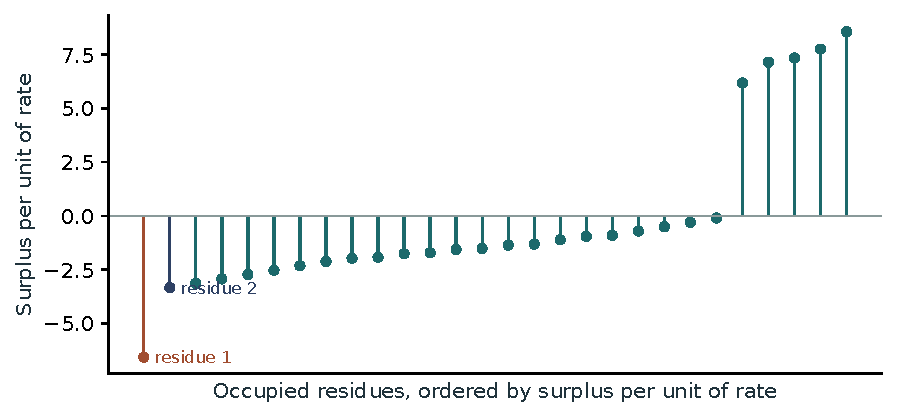
\includegraphics[width=.90\linewidth]{figures/rates.pdf}
\caption{On the adverse order of the previous support rule, each vertical segment is a leaf's coefficient \(p_t-zq_t\) at the optimized standard target. Rates should be exchanged according to differences between these heights. Leaf 1 has the lowest height but must supply marks. Leaf 2 can absorb the count adjustment.}\label{fig:rate-ledger}
\end{figure}

The large change since the previous paper came from freeing the allocation on the surviving leaves. Restoring the trial-count prefactor subsequently gains only about \(0.0000356\) percentage points. It would be misleading to ascribe the first improvement to a weakened admissibility test, or to use the second as evidence that a particular support exchange helped on every order. The next experiment changes the actual positions and keeps an explicit fallback wherever its new supports cannot certify a higher fraction.
